\question 对一个无噪声的4kHz信道进行采样,可达到的最大数据传输速率是( )
\par\twoch{4kbit/s}{8kbit/s}{1kbit/s}{\textcolor{red}{无限大}}
\begin{solution}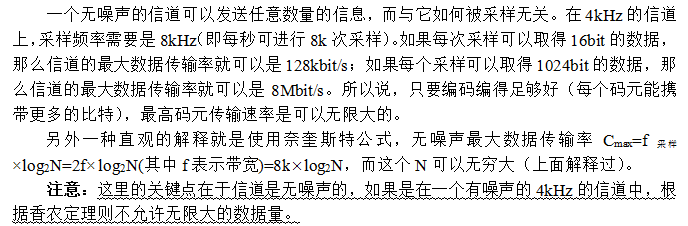
\includegraphics[width=3.70833in,height=1.21875in]{computerassets/B0AE585B95CFFFFD9D175FCB4B196857.png}
\end{solution}
\question 一个信道每1/8s采样一次,传输信号共有16种变化状态,则最大数据传输速率是(
)
\par\twoch{16bit/s}{\textcolor{red}{32bit/s}}{48bit/s}{64bit/s}
\begin{solution}信道每1/8s采样一次,说明采样频率为8Hz。由采样定理可知,采样频率必须大于或等于最大频率的两倍。也就是说,此信道的最高频率为4Hz,既然是要求最大数据传输速率,不妨设最小频率为0Hz,那么就可以求出最大带宽=最高频率-最低频率=4Hz。于是就可以使用奈奎斯特定理来计算,即最大数据传输速率=2×4×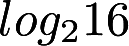
\includegraphics[width=0.46875in,height=0.15625in]{texmath/8d88685Cdpi7B3507Dlog_216}=32bit/s。当然,此题也可以直接使用公式:Cmax=f采样×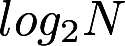
\includegraphics[width=0.45833in,height=0.14583in]{texmath/b7c31d5Cdpi7B3507Dlog_2N}=8×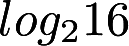
\includegraphics[width=0.46875in,height=0.15625in]{texmath/8d88685Cdpi7B3507Dlog_216}=32bit/s。
\end{solution}
\question 假设一个无噪声的信道,带宽是6MHz,并且采用了4级数字信号,那么它每秒可发送的数据量为(
)
\par\twoch{6Mbit}{12Mbit}{\textcolor{red}{24Mbit}}{48Mbit}
\begin{solution}根据奈奎斯特定理,可以对信道每秒采样12M次。因为是4级数字信号,每次采样可获得2bit的数据,所以总共的数据传输率是24Mbit/s,即每秒发送了24Mbit的数据。
提醒:4级数字信号指什么?这个无需知道,在考研中,只需记住一点,看到这种条件,直接log2即可,得到有用的信息。
\end{solution}
\question 在无噪声的情况下,若某通信链路的带宽为3kHz,采用4个相位、每个相位具有4种振幅的QAM调制技术,则该通信链路的最大数据传输速率是(
)
\par\twoch{12kbit/s}{\textcolor{red}{24kbit/s}}{48kbit/s}{96kbit/s}
\begin{solution}首先,题干已经很明确地说明是在无噪声的信道,所以锁定解答此题的公式为奈奎斯特定理。解答此题的步骤,一般是先算出最大波特率,题目中已经给出带宽为3kHz,由总结中给出的公式可知最大的波特率为2×3kHz=6kBaud。只要算出了最大波特率,接下来只需计算一个码元携带多少比特即可。题干说了采用4个相位,并且每个相位有4种振幅,也就是说可以表示16种状态,所以一个码元可以携带4bit(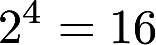
\includegraphics[width=0.56250in,height=0.16667in]{texmath/aaccb55Cdpi7B3507D25E43D16})的信息,故该通信链路的最大数据传输速率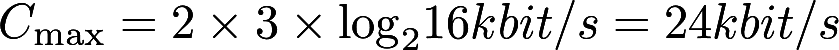
\includegraphics[width=3.00000in,height=0.17708in]{texmath/5dd0b05Cdpi7B3507D7BC_7B5Cmax7D7D3D25Ctimes35Ctimes7B5Clog_27D16kbit2Fs3D24kbit2Fs}。
提醒:一个码元携带多少比特有非常多的方式给出,如本题是通过QAM调制技术给出,考生无需理解QAM调制技术是什么,只需算出总状态的个数N,求出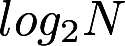
\includegraphics[width=0.45833in,height=0.14583in]
{texmath/b7c31d5Cdpi7B3507Dlog_2N}
即可。
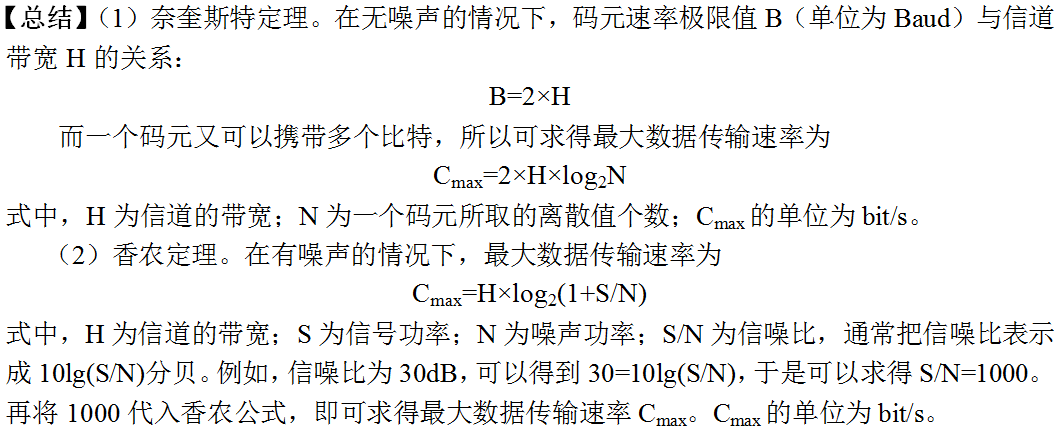
\includegraphics[width=3.46875in,height=1.40625in]{computerassets/C4BCB29C720DA803C2491CE5A88154C0.png}
\end{solution}
